\section*{Экспериментальные результаты}

Для получения коэффициента преобразования $K_H = \frac{H}{X}$, где $X$ -- отклонение по горизонтальной оси осциллографа в делениях, воспользуемся формулой \ref{eq:H_tor}. Учитывая, что $I = \frac{X \cdot K_X}{R_0}$, получим:
$$ K_H = \frac{K_X}{R_0} \frac{N_0}{2 \pi R}.$$
Для $K_B = \frac{B}{Y}$, где $Y$ -- отклонение по вертикальной оси осциллографа, воспользуемся \ref{eq:B_circuit}:
$$ K_B = \frac{\tau_{\text{и}}}{SN_u} K_Y.$$
Значение $\tau_{\text{и}}$ определяется параметрами интегрирующей цепочки:
$$ \tau_{\text{и}} = RC = 20 \; \text{кОм} \cdot 20 \; \text{мкФ} = 0.4 \; \text{с}. $$
Данное значение также было проверено экспериментально с помощью осциллографа.

Найдем амплитуду $H_{max}$ колебаний напряженности поля в тороиде в условиях насыщения и индукцию насыщения $B_s$. Также определим их отношение для оценки усиления поля в образце.

По положениям точек пересечения кривых с осями координат определим коэрцитивное поле $H_c$ и остаточную индукцию $B_r$. Для них тоже определим их отношение.

Полученные результаты сведены в таблицу \ref{tab:results}.

\begin{table}[H]
	\centering
	\footnotesize
	\input{../gen/tab_results.tex}
	\caption{Параметры петель гистерезиса}
	\label{tab:results}
\end{table}

Плавно уменьшая силу тока через образец определим начальную кривую намагничивания для образцов. Также приведем графики предельных петель гистерезиса (см рис. \ref{img:ferrit}, \ref{img:fesi}, \ref{img:feni}).

\begin{figure}[H]
	\centering
	\begin{minipage}[c]{.43\textwidth}
		\centering
		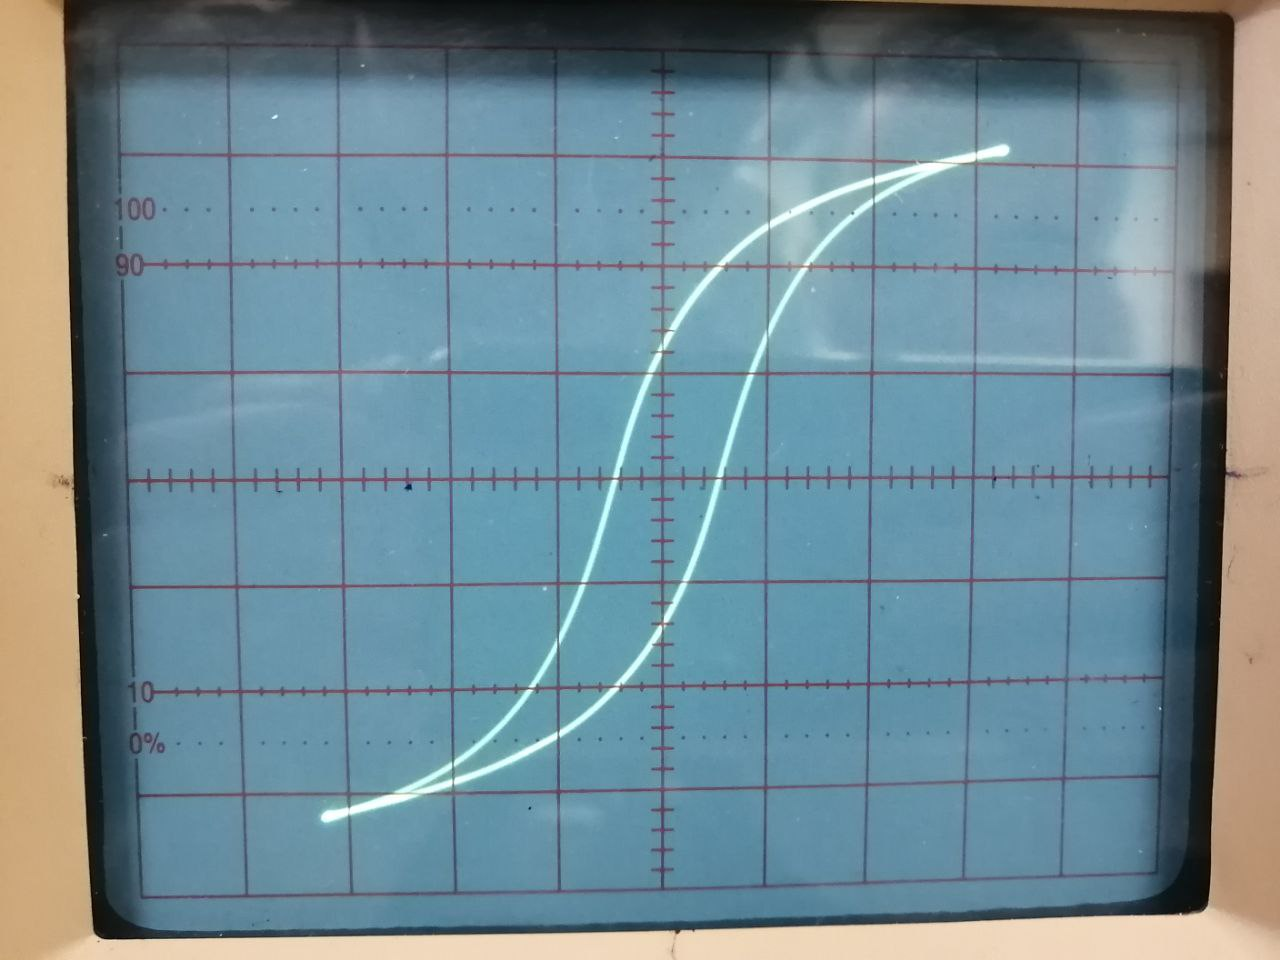
\includegraphics[width=0.9\linewidth]{"../photos/ferrit.jpg"}
		\caption*{Предельная петля}
	\end{minipage}%
	\begin{minipage}[c]{.57\textwidth}
		\centering
		\includegraphics[width=0.9\linewidth]{"../gen/Ferrit_B_H.pdf"}
		\vspace{-10pt}
		\caption*{Начальная кривая намагничивания}
	\end{minipage}
	\caption{Феррит}
	\label{img:ferrit}
\end{figure}

\begin{figure}[H]
	\centering
	\begin{minipage}[c]{.43\textwidth}
		\centering
		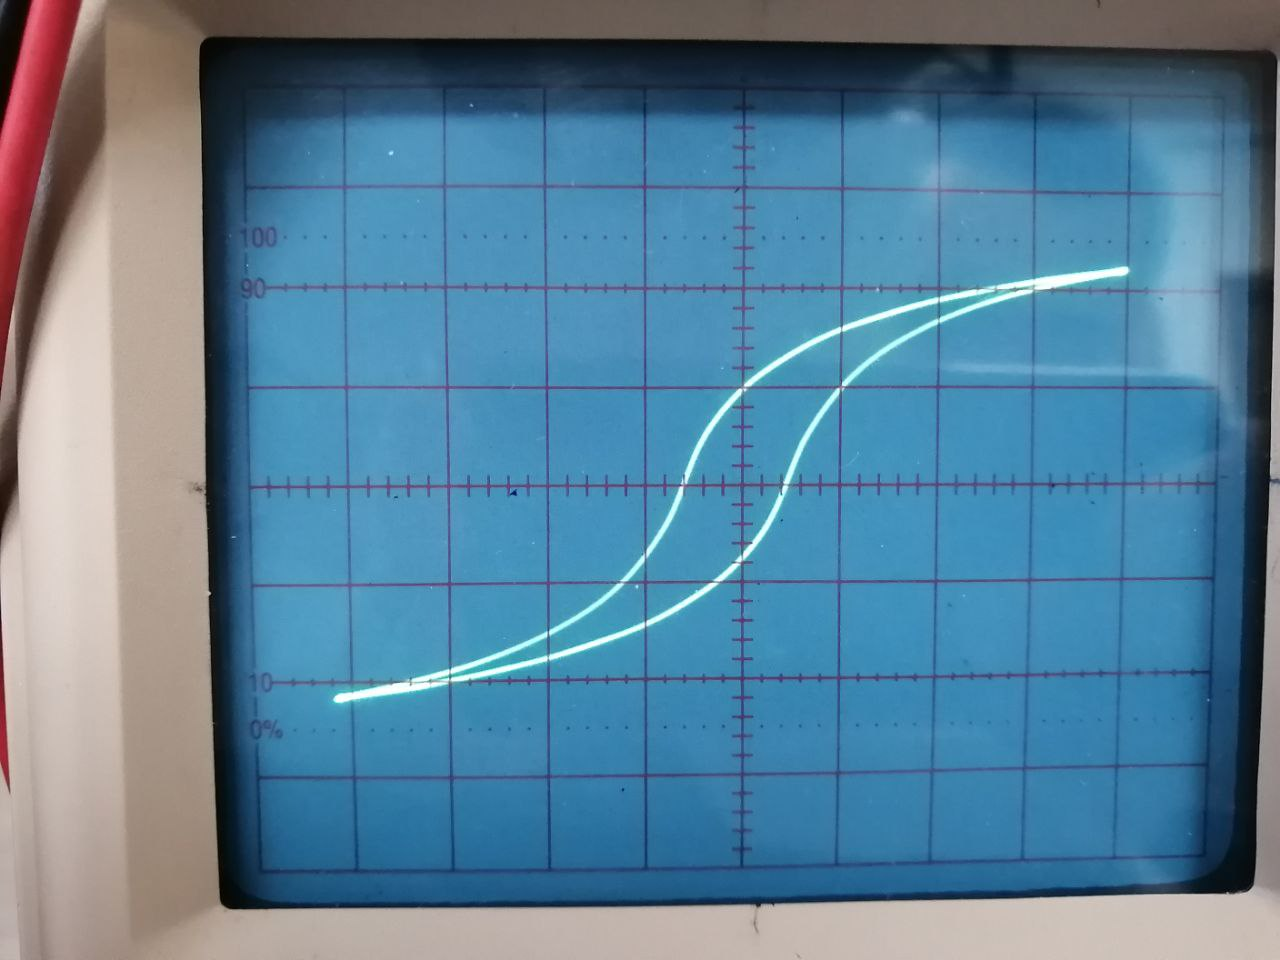
\includegraphics[width=0.9\linewidth]{"../photos/fe_si.jpg"}
		\caption*{Предельная петля}
	\end{minipage}%
	\begin{minipage}[c]{.57\textwidth}
		\centering
		\includegraphics[width=0.9\linewidth]{"../gen/Fe-Si_B_H.pdf"}
		\vspace{-10pt}
		\caption*{Начальная кривая намагничивания}
	\end{minipage}
	\caption{Кремнистое железо}
	\label{img:fesi}
\end{figure}

\begin{figure}[H]
	\centering
	\begin{minipage}[c]{.43\textwidth}
		\centering
		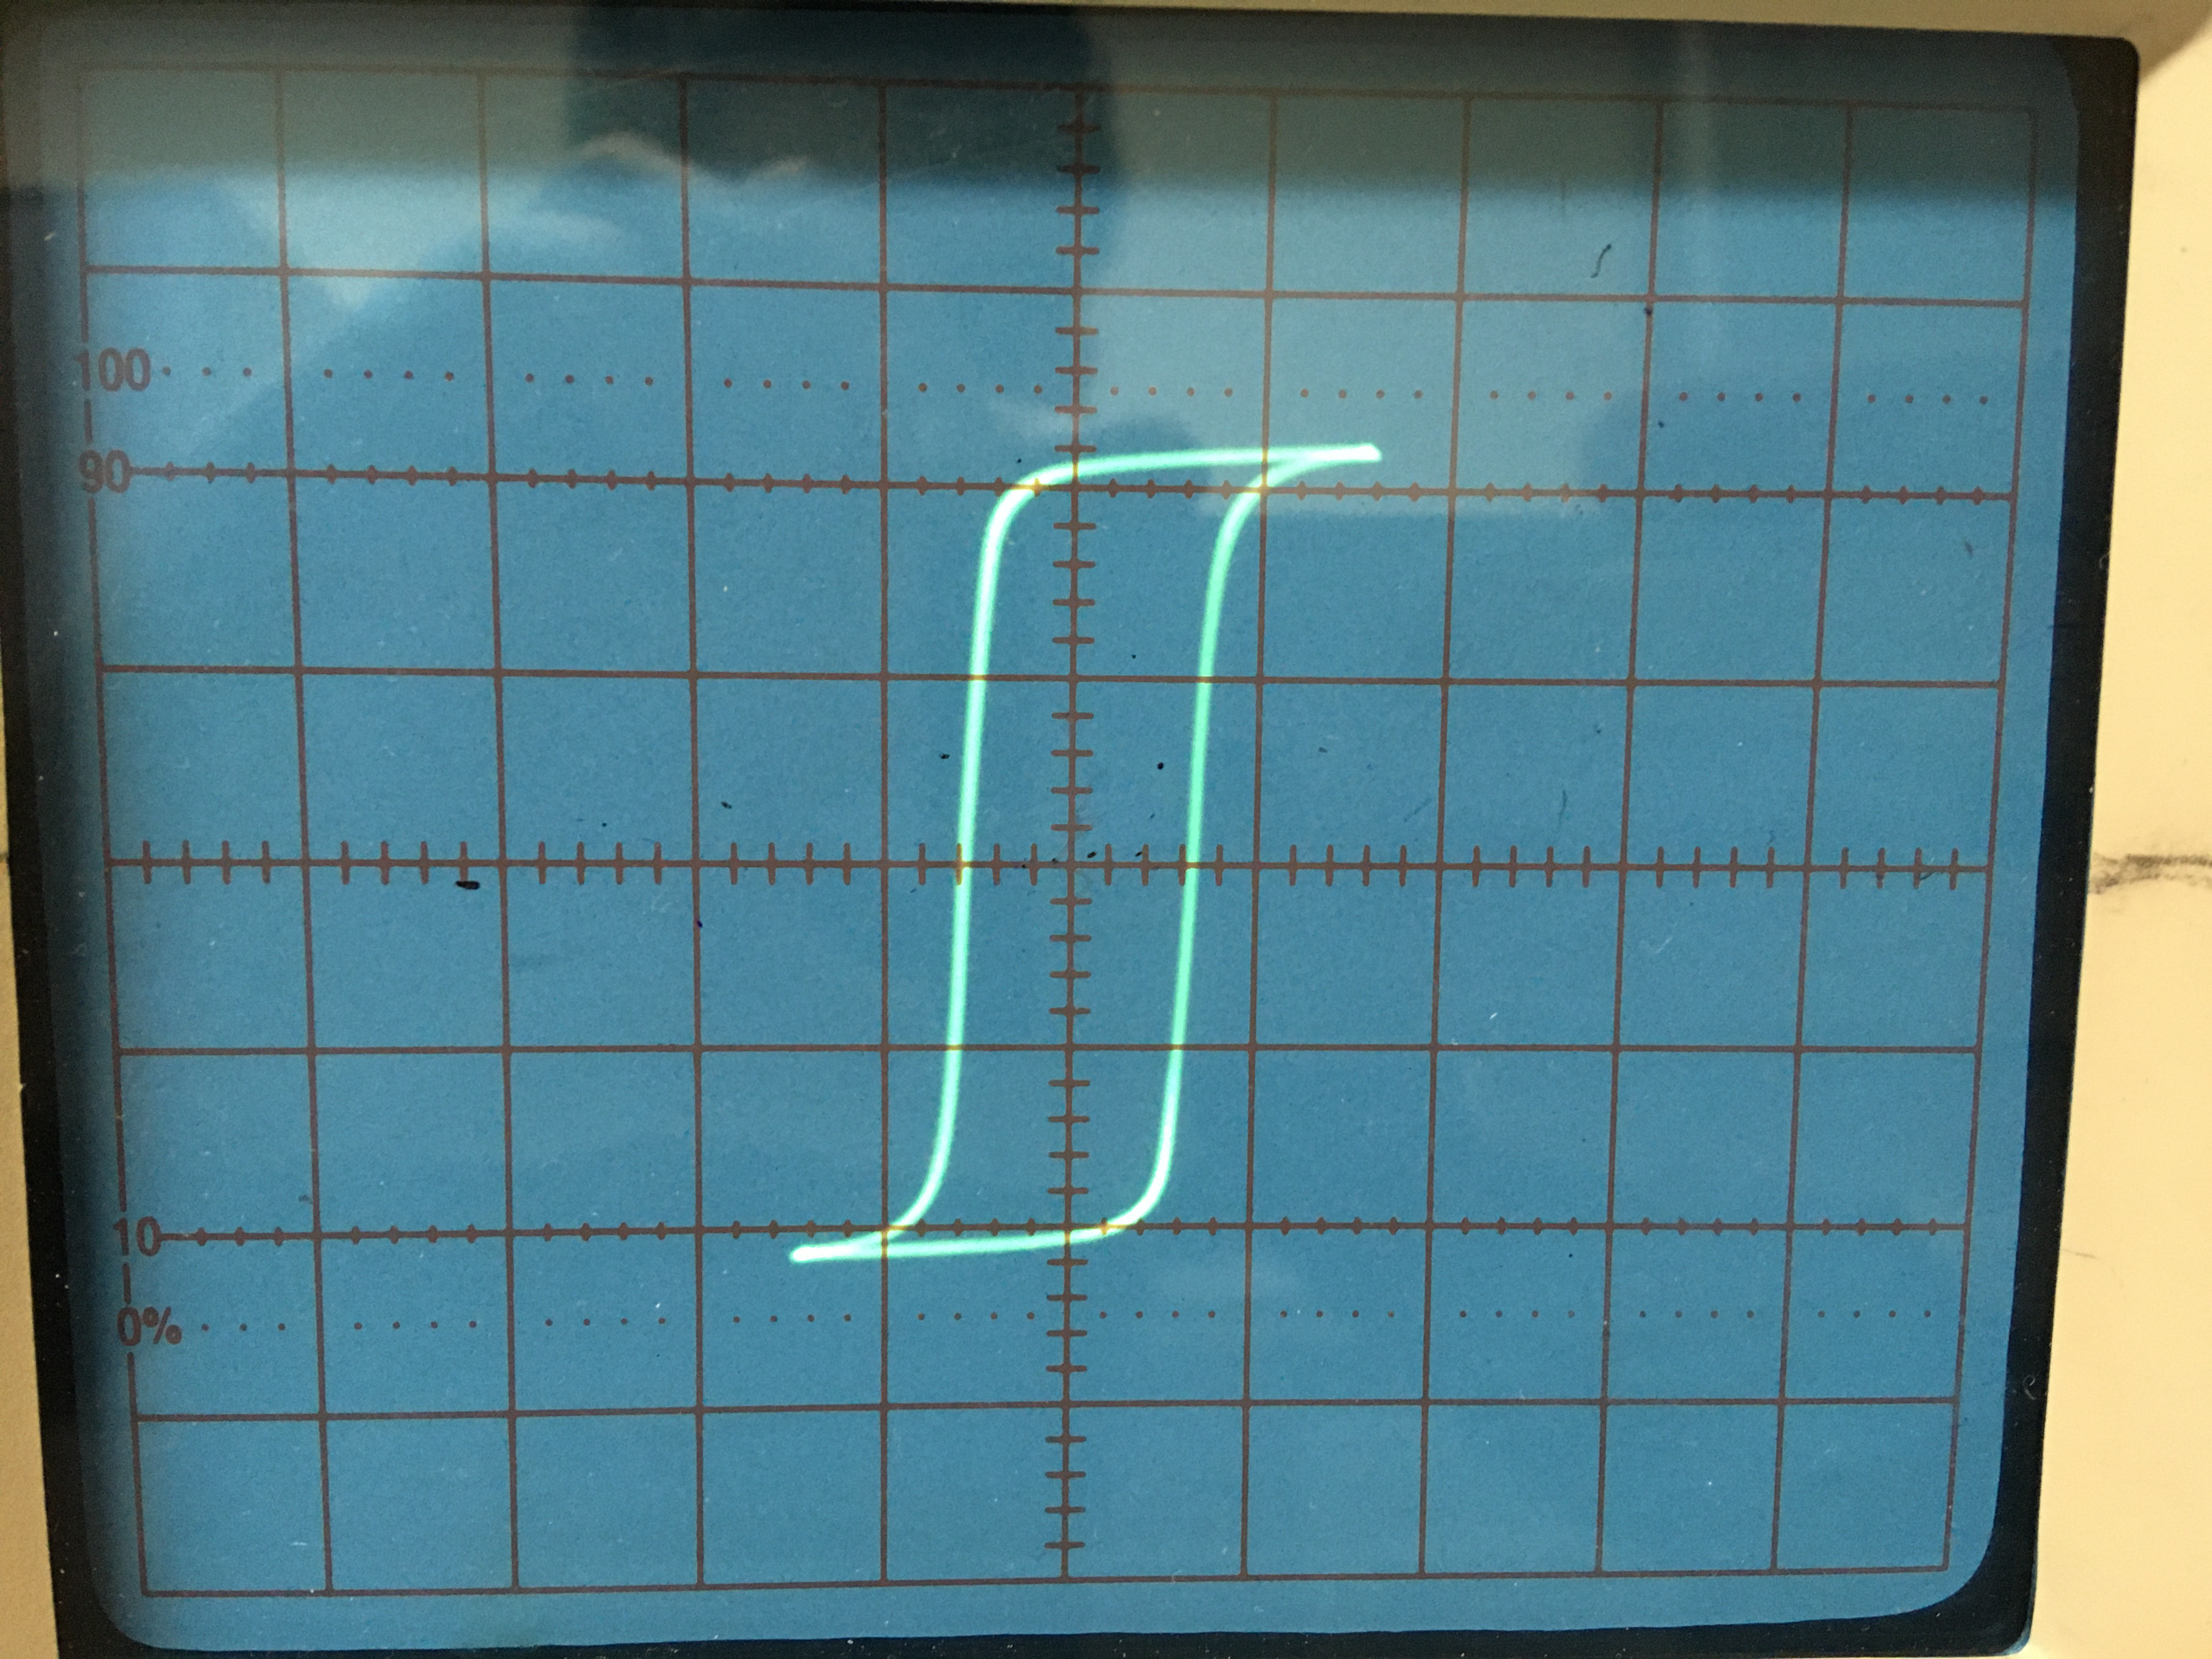
\includegraphics[width=0.9\linewidth]{"../photos/fe_ni.jpg"}
		\caption*{Предельная петля}
	\end{minipage}%
	\begin{minipage}[c]{.57\textwidth}
		\centering
		\includegraphics[width=0.9\linewidth]{"../gen/Fe-Ni_B_H.pdf"}
		\vspace{-10pt}
		\caption*{Начальная кривая намагничивания}
	\end{minipage}
	\caption{Пермаллой}
	\label{img:feni}
\end{figure}

Из графиков определим значения дифференциальных магнитных проницаемостей $\mu$ в начале координат и в точке максимума. Для сравнения приведем справочные значения магнитных проницаемостей.

\begin{table}[H]
	\centering
	\footnotesize
	\input{../gen/tab_diff.tex}
	\caption{Дифференциальные магнитные проницаемости}
	\label{tab:diff}
\end{table}
